\setlength{\tabcolsep}{1pt}
\begin{figure}[h]
    \footnotesize
    \small
    \centering
    % \begin{tabular}{*{6}{p{2.8cm}}}
    %   \hline
    %   & & & & & \\
    %   \centering Input & \centering \ptopzero & \centering \nulltext & \centering  \directinversion & \centering  \negprox & \centering \method{} \\
    %   %   \multicolumn{6}{c}{``\textit{A \textcolor{RoyalBlue}{\textbf{lego}} cat \textcolor{RoyalBlue}{\textbf{toy}} sitting next to a mirror}"} \\
    %   \multicolumn{6}{c}{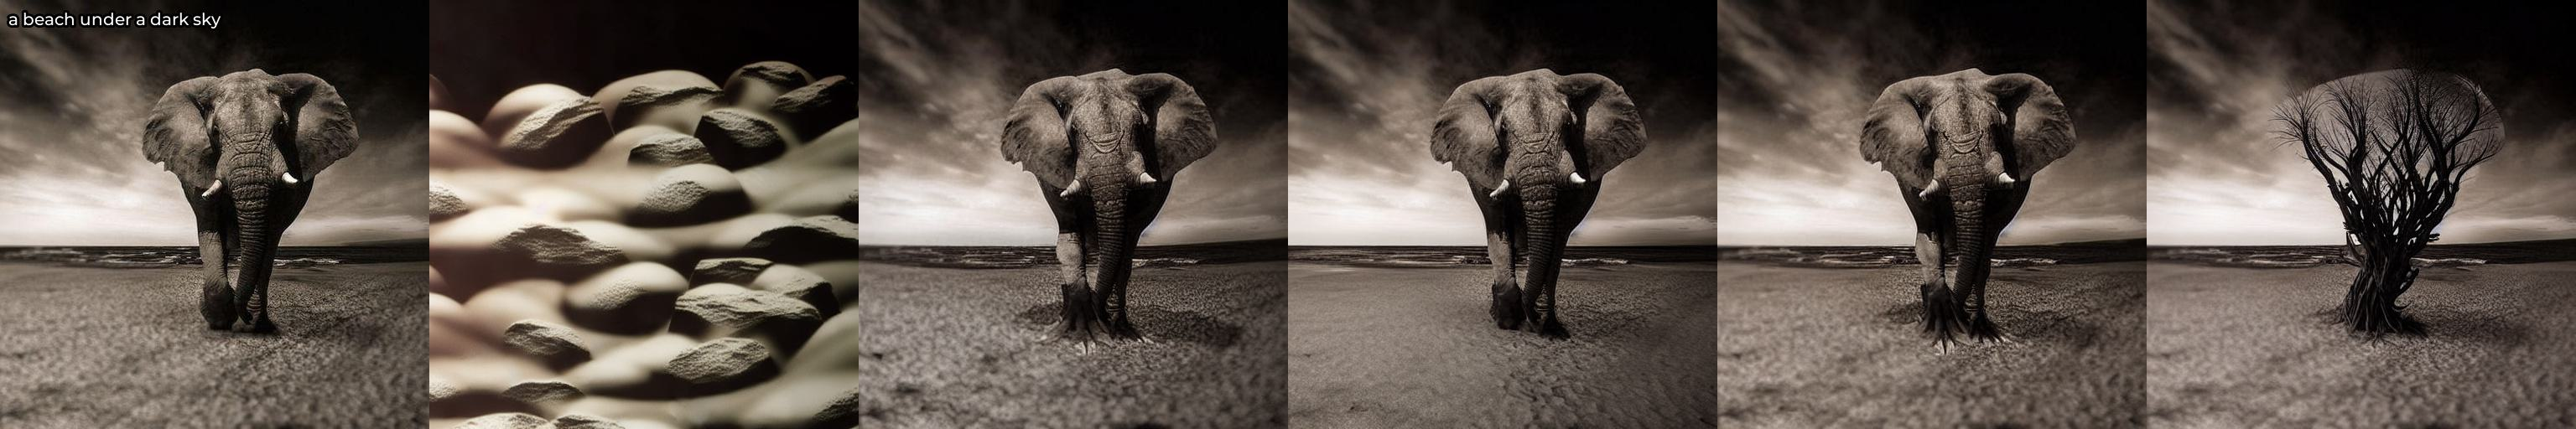
\includegraphics[width=\linewidth]{fig/ex_structpres/3_delete_object_80-2_natural-1_animal-321000000005}} \\
    % \multicolumn{6}{c}{}  \\
    % % 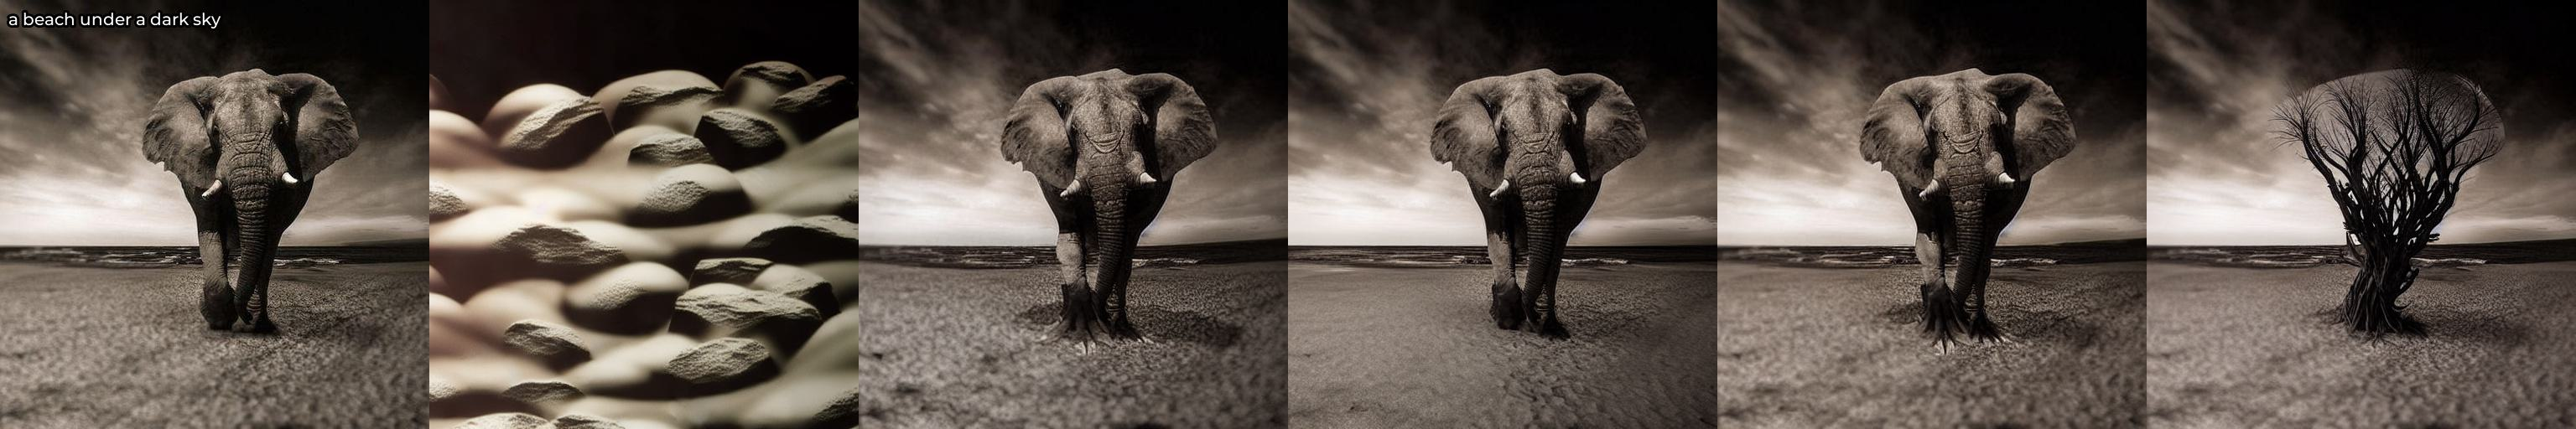
\includegraphics[height=2.2cm]{fig/ex_structpres/3_delete_object_80-2_natural-1_animal-321000000005} \\
    % %   \multicolumn{6}{c}{``\textit{Orange van with \textcolor{BrickRed}{\st{surfboards}} \textcolor{RoyalBlue}{\textbf{flowers}} on top}"} \\
    % %   \insertimage{van}{input}\\
    % %   \multicolumn{6}{c}{``\textit{Meat \textcolor{BrickRed}{\st{balls}} \textcolor{RoyalBlue}{\textbf{shushi}} on white plate}"} \\
    % %   \insertimage{meat}{input}\\
    % %   \multicolumn{6}{c}{``\textit{A \textcolor{BrickRed}{\st{woman}} \textcolor{RoyalBlue}{\textbf{storm-trooper}} with blue hair}"} \\
    % %   \insertimage{girl}{input}\\
    % %   \multicolumn{6}{c}{``\textit{A \textcolor{BrickRed}{\st{cat}} \textcolor{RoyalBlue}{\textbf{dog}} sitting on a wooden chair}"} \\
    % %   \insertimage{cat2}{input}\\
    %   \hline
    %   % ... Add more rows as needed
    % \end{tabular}
    \begin{tabularx}{0.7\columnwidth}{ YYYY }
        VAE & \method &  VAE & \method  \\
        
\includegraphics[width=\linewidth]{fig/reconstruction/000000000040_vae.png} & 
\includegraphics[width=\linewidth]{fig/reconstruction/000000000040.png} &
        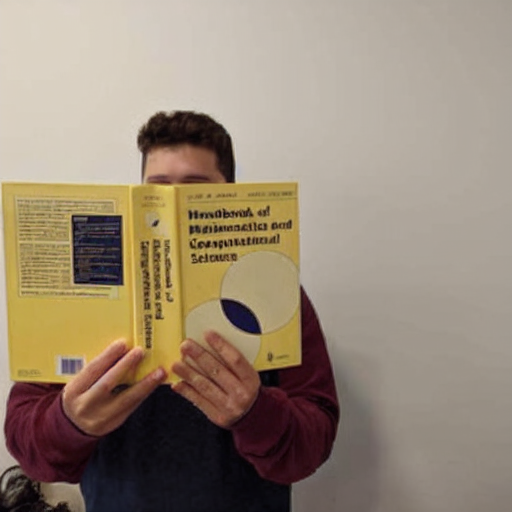
\includegraphics[width=\linewidth]{fig/reconstruction/223000000000_vae.png} & 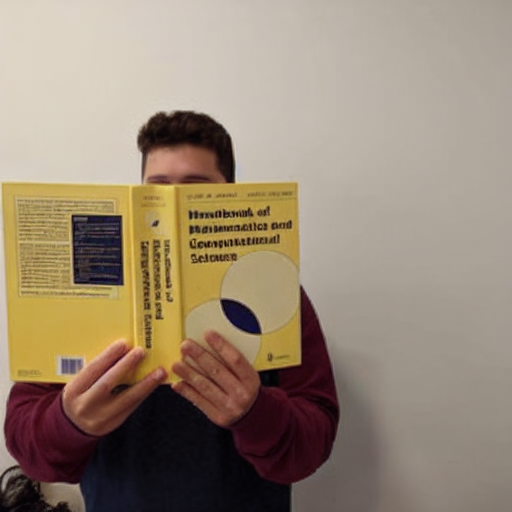
\includegraphics[width=\linewidth]{fig/reconstruction/223000000000.png}
        \\
        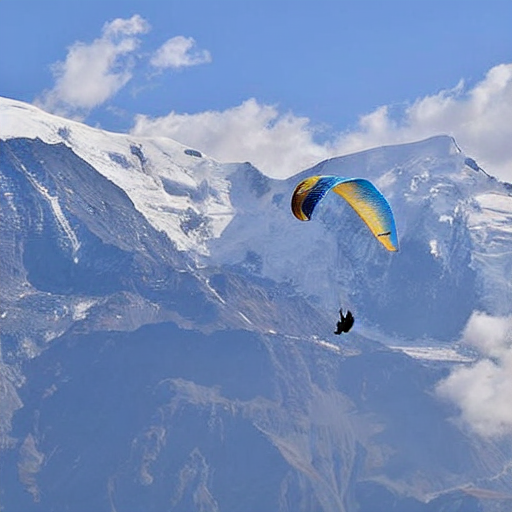
\includegraphics[width=\linewidth]{fig/reconstruction/324000000002_vae.png} & 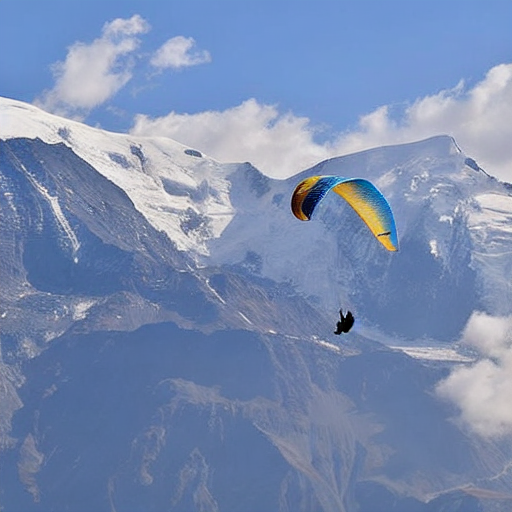
\includegraphics[width=\linewidth]{fig/reconstruction/324000000002.png} &
        
\includegraphics[width=\linewidth]{fig/reconstruction/412000000004_vae.png} & 
\includegraphics[width=\linewidth]{fig/reconstruction/412000000004.png}
        \\
        \end{tabularx}
    \caption{Reconstruction performance on PieBench samples.}
    % \caption{This figure displays examples where \method{} successfully removes objects from images, a feature not commonly observed in other negative-prompt-based methods. Each example illustrates how the removed element is replaced with content that, unexpectedly, shares structural similarities with the original object. This phenomenon, resulting from the interplay between CFG and SA guidance, highlights a unique aspect of our method's behavior and an opportunity for further refinement.} 
    \label{fig:res_reconstruction}
  \end{figure}